\documentclass[12pt,a4paper]{article}
\usepackage{../../../template/stile}

%Titolo documento
\newcommand{\titoloDocumento}{Norme di Progetto}

%Prima data di creazione del documento
\newcommand{\dataCreazione}{30 novembre 2015}

%Inserite la versione attuale del documento
\newcommand{\versione}{1.0.3}

%Stato in cui si trova il documento: Formale solo all'atto di consegna
\newcommand{\stato}{Informale}

%Uso del documento
\newcommand{\uso}{Interno}

\rhead{\titoloDocumento}
\lfoot{Versione: \versione}
\title{\titoloDocumento}

\begin{document}
\begin{titlepage}
\begin{center}
\today \\
\vspace{1cm}
\begin{Huge}
\textbf{\nomeGruppo} \\
\end{Huge}
\textbf{\prjL} \\
\vspace{1cm}

\includegraphics[scale=0.5]{\logoGrande}
\vspace{1cm}

\HRule \\[0.4cm]
\begin{Huge}
{\huge \bfseries \titoloDocumento}\\[0.4cm]
\end{Huge}
\HRule \\[1cm]
\vfill

\begin{table}[h]
\begin{center}
\begin{tabular}{r | l}
\multicolumn{2}{c}{\textbf{Informazioni sul documento}}\\
\midrule
\textbf{Nome Documento}	&	\titoloDocumento	\\
\textbf{Versione}	&	\versione	\\
\textbf{Stato}	&	\emph{\stato}	\\
\textbf{Uso}	&	\emph{\uso}	\\
\textbf{Data Creazione}	&	\dataCreazione	\\
\textbf{Data Ultima Modifica}	&	\today	\\
\textbf{Redazione}	&	\NDC	\\
\ &	\AVE	\\
\ &	\AVI	\\
\textbf{Verifica}	&	\IB	\\
\ & \TP \\
\textbf{Approvazione}	&	\AB	\\
\textbf{Lista Distribuzione}	&	\nomeGruppo	\\

\end{tabular}
\end{center}
\end{table}

\end{center}
\end{titlepage}
\newpage

\Large{\textbf{Registro delle modifiche}}
\normalsize

\begin{table}[h]
\begin{center}

\begin{tabular}{p{0.12\textwidth} p{0.2\textwidth} p{0.18\textwidth} p{0.39\textwidth}}
\toprule
\textbf{Versione}	&	\textbf{Autore}	&	\textbf{Data}	&	\textbf{Descrizione}\\
\midrule
\midrule
1.0.5 & \AVE & 2015-12-10 & Ticketing \\
\midrule
1.0.4 & \AVE & 2015-12-08 & Ruoli di progetto e Riunioni \\
\midrule
1.0.3 & \AVI & 2015-12-07 & Norme del Piano di Progetto e dell'Analisi dei requisiti \\
\midrule
1.0.2 & \AVI & 2015-12-03 & Descrizione processi di base \\
\midrule 
1.0.1 & \NDC & 2015-12-02 & Introduzione \\
\midrule
1.0.0 & \NDC & 2015-11-30 & Template di base \\
\bottomrule
\end{tabular}
\caption{Versionamento del documento}
\label{tabVers1}
\end{center}
\end{table}
\newpage

\tableofcontents
\newpage

\listoftables
\listoffigures
\newpage

% NOTA non so dove mettere l'uso di git

\section{Introduzione}
Questo documento definisce le norme che i membri del gruppo \nomeGruppo{} adotteranno nello svolgimento del progetto \prjL. Tutti i membri sono tenuti a leggere il documento attentamente e a seguirne le norme.

\subsection{Scopo}
Il documento si propone come proposito di garantire l'uniformità di tutto il materiale prodotto, migliorarne l'efficienza e ridurne gli errori.

\subsection{Descrizione}
Verranno definite norme riguardanti:
\begin{itemize}
  \item interazioni tra membri del gruppo;
  \item stesura documenti, convenzioni stilistiche e tipografiche;
  \item modalità di lavoro durante tutte le fasi del progetto;
  \item ambiente di lavoro.
\end{itemize}

\subsection{Glossario}
Al fine di evitare ogni ambiguità di linguaggio e massimizzare la comprensione dei
documenti, i termini tecnici, di dominio, gli acronimi e le parole che necessitano chiarimenti sono riportate nel documento \emph{Glossario\_v1.2.0}. Ogni occorrenza di vocaboli presenti nel \GlO è marcata da una G maiuscola in pedice (e.g. \gloss{pedice}).

\newpage

\section{Processi base} %ISO 12207 5
I processi base sono formati dai seguenti sotto processi:
\begin{enumerate}
\item Processo dell'acquirente
\item Processo del fornitore
\item Processo di sviluppo
\item Processo operativo
\item Processo di manutenzione
\end{enumerate}
Per lo scopo del corrente progetto saranno dettate solo le norme per le fasi del fornitore e di sviluppo, poiché i processi  dell'acquirente non riguardano il team e le fasi operative e di manutenzione non verranno trattate.

\subsection{Processi del fornitore}

\subsubsection{Scopo}
Definisce le attività e i task attraverso i quali il fornitore comunica al committente modo, tempi e costi previsti per il progetto.

\subsubsection{Descrizione}
Consiste nel redigere il \PdQ, che dovrà illustrare la strategia complessiva di verifica e validazione proposta dal fornitore per pervenire al collaudo del sistema con la massima efficienza ed efficacia, e il \PdP, che dovrà presentare l'organigramma dettagliato del fornitore, lo schema proposto per l'assegnazione e la rotazione dei ruoli di progetto, l'impegno complessivo previsto per ogni ruolo e per ogni individuo, e il conto economico preventivo di realizzazione del prodotto. Le regole dettagliate per redigere il \PdP\ verranno analizzate nel prossimo paragrafo.

\subsubsection{Piano di Progetto} %ISO 12207 5.2.4
Il \PM, assieme all'\AM, deve presentare nel \PdP\ diagrammi di Gant e ripartizione delle risorse relativi ad ogni fase del Progetto. In Particolare è necessario che ogni componente del gruppo ricopra tutti i ruoli nell'arco dello svolgimento del progetto. La rotazione dei ruoli deve garantire un'equa ripartizione del carico di lavoro individuale, ovvero il totale di ore produttive per ogni persona può differire al più di poche unità da quello degli altri. Inoltre è possibile che un componente rivesta più ruoli contemporaneamente, ma sempre evitando conflitti di interesse. In particolare i conflitti di interesse da evitare sono quelli tra \PM\ e qualsiasi altro ruolo o tra \VR\ e qualsiasi altro ruolo.

\subsection{Processi di sviluppo}

\subsubsection{Scopo}
Il processo di sviluppo produce un prodotto software che soddisfi i requisiti architetturali. Inoltre definisce un insieme di azioni che formalizzano comportamenti, interfacce e vincoli di implementazione atti a creare un prodotto software

\subsubsection{Descrizione}
Il processo di sviluppo è un insieme di attività e task necessari per lo sviluppo di un prodotto software. Coloro che eseguono queste attività' sono gli sviluppatori. Le attività che compongono i processi di sviluppo sono:
\begin{enumerate}
\item Processo di Analisi dei requisiti
\item Processo di Progettazione
\item Processo di Codifica
\end{enumerate}

\subsubsection{Analisi dei requisiti} %ISO 12207 5.3.2

\paragraph{Scopo}
Gli Analisti dovranno produrre l'Analisi dei Requisiti basandosi sul capitolato e sugli incontri con il proponente. Tale processo ha l'obiettivo di formalizzare e rendere tracciabile in un documento i requisiti e casi d'uso individuati, comprendendo a fondo eventuali problemi da risolvere in fase di progettazione.

\paragraph{Descrizione}
Con il completamento di questo processo si ottiene una documentazione affidabile e consistente che ben descrive le esigenze e le richieste del proponente.

\paragraph{Casi d'uso}
I casi d'uso sono creati secondo lo standard UML 2.0 e sono identificati dalla seguente notazione:
\begin{center}
UC[codice] - [Titolo]
\end{center}
dove il \textbf{codice} è un numero progressivo identificativo di ogni requisito, gerarchico nel  caso di sotto-casi d'uso tramite la notazione \textit{CodiceUCPadre.CodiceSottoUC}. Per ogni caso d'uso deve inoltre essere indicato:
\begin{itemize}
\item \textbf{Titolo} breve ma non ambiguo
\item \textbf{Attori} principali e secondari coinvolti
\item \textbf{Descrizione} sintetica del Caso d'uso
\item \textbf{Precondizione}
\item \textbf{Postcondizione}
\item \textbf{Requisiti} collegati al Caso d'uso
\end{itemize}

\paragraph{Classificazione dei Requisiti}
È compito degli Analisti stilare una lista dei requisiti emersi dal capitolato e da eventuali
riunioni con il proponente. Questi requisiti dovranno essere classificati per tipo e
importanza, utilizzando la seguente codifica:
\begin{center}
R[importanza][tipo][codice]
\end{center}
\begin{itemize}
\item \textbf{Importanza} può assumere i seguenti valori:
\begin{description}
\item[0:] Requisito obbligatorio
\item[1:] Requisito desiderabile
\item[2:] Requisito opzionale
\end{description}
\end{itemize}
\begin{itemize}
\item \textbf{Tipo} può assumere i seguenti valori:
\begin{description}
\item[F:] Funzionale, descrive i servizi o le funzioni offerte dal sistema
\item[N:] Non funzionale, descrivono i vincoli sui servizi offerti dal sistema
\end{description}
\end{itemize}
\begin{itemize}
\item \textbf{Codice} è un numero progressivo univoco per ogni requisito, indipendente da importanza e tipo. Nel caso si abbia un sotto-requisito codice può anche essere espresso in modo gerarchico tramite la notazione \textit{CodiceRequistoPadre.CodiceSottorequisito}
\end{itemize}
Ogni requisito deve essere correlato da una sintetica ma precisa descrizione

\subsubsection{Progettazione}
Le norme di progetto saranno ampliate con questa sezione non appena verranno concordate dal gruppo.

\subsubsection{Codifica}
Le norme di progetto saranno ampliate con questa sezione non appena verranno concordate dal gruppo.

\newpage

\section{Processi di Supporto} %ISO 12207 6

\subsection{Scopo}
Definisce norme per lo sviluppo e il mantenimento della documentazione prodotta durante il ciclo di vita del software. Inoltre definisce metodi per il controllo della qualità, di verifica e validazione di tali documenti.

\subsection{Descrizione}
Verranno definite norme riguardanti:
\begin{itemize}
  \item utilizzo e l'accesso ai documenti;
  \item templates da utilizzare, l'uniformità di linguaggio, le convenzioni stilistiche e tipografiche;
  \item metodi di verifica e approvazione dei documenti;
\end{itemize}

\subsection{Documentazione}\label{Documentazione} %ISO 12207 6.1
La readazione di tutti i documenti viene assegnata dal \PM{} ai responsabili della stesura di tale documento secondo i \gloss{ruoli} definiti nella sezione \ref{Ruoli}. Successivamente se i redattori ritengono che il documento sia completo, su comferma da parte del \PM, il documento deve essere preso in visione da un \VR. Se il \VR ritiene che documento rispetta i requisiti imposti dal \PR{} e supera il controllo di qualità può proporre al \PM{} l'approvazione di tale documento. Se il documento viene approvato è giunto alla fase finale.

Tutti documenti essi dovranno a essere denominati secondo il seguente formalismo:
\begin{center}
\emph{NomeDocumento\_vX.Y.Z.pdf}
\end{center}
dove \emph{NomeDocumento} rappresenta il nome del documento e \emph{vX.Y.Z} la versione come spiegata nella sezione \ref{Versione}. Il documento non può contenere lettere accentate. Nel caso il nome fosse composto da più parole, la prima lettera di ogni parola deve essere maiuscola e non devono esserci spazi, \emph{underscore} o trattini a separare le parole.

Ogniqualvolta sia necessaria la citazione di una versione specifica di un documento, essa deve comprendere sia il nome che il numero di versione aderente al formato:
\begin{center}
\emph{Nome Documento vX.Y.Z}
\end{center}

\subsubsection{Versione} \label{Versione}
La documentazione prodotta deve essere corredata del numero di versione attuale tramite la seguente codifica \emph{vX.Y.Z} dove:
\begin{itemize}
  \item \textbf{X} indica il numero crescente di uscite formali del documento. All'inizio di ogni fase il \PM deve cambiare tale indice seguendo la numerazione progressiva indicata e impostare a 0 gli indici Y e Z. L'indice deve seguire la numerazione progressiva indicata e non sono ammessi indici diversi da quelli elencati:
  \begin{enumerate}
    \item fase che si conclude con la \RR;
    \item fase che si conclude con la \RP;
    \item fase che si conclude con la \RQ;
    \item fase che si conclude con la \RA;
  \end{enumerate}
  \item \textbf{Y} indica la fase in cui il documento si trova. Nel momento in cui inizia l'attività di stesura il redattore del documento deve controllare che tale indice sia correttamente impostato a 0. All'inizio della verifica il \VR{} deve variare l'indice impostandolo a 1, dopo aver ricevuto il consenso dal \PM. Conclusa la verifica, il \PM{} provvede all'approvazione del documento e deve impostare l'indice a 2. L'indice deve seguire la numerazione progressiva indicata e non sono ammessi indici diversi da quelli elencati:
  \begin{enumerate}[start=0]
    \item stesura del documento;
    \item verifica del documento;
    \item approvazione del documento.
  \end{enumerate}
  \item \textbf{Z} indica il numero crescente di modifiche minori. Ad ogni modifica effettuata deve corrispondere ad un'aggiunta di una voce nel diario delle modifiche, il redattore o il \VR devono aggiornare l'indice seguendo una numerazione progressiva. Non viene fissato un limite superiore per tale indice.
\end{itemize}

\subsubsection{Stato}
I documenti sono provvisti di uno \gloss{stato}. Tale stato può essere \gloss{informale} o  \gloss{formale}.

\subsubsubsection{Informale}
Tutti i documenti saranno da ritenersi informali fino all'approvazione del \PM, il quale potrà richiederne una revisione ulteriore. L'utilizzo dei documenti informali è da considerarsi esclusivamente interno al gruppo e localizzato durante la fase di redazione e verifica di tali documenti.

\subsubsubsection{Formale}
I documenti approvati dal \PM{} si riterranno formali e pronti per essere distribuiti. Solo i documenti formali potranno essere distribuiti alla loro lista di distribuzione. Ogniqualvolta un documento formale venga modificato o rivisitato, la nuova versione è da considerarsi non formale fino ad approvazione del \PM e quindi sarà trattata come un documento informale.

\subsubsection{Uso}
I documenti possono avere diverse liste di distribuzione ma una devono essere classificati in due principali categorie: uso interno ed esterno.

\subsubsubsection{Interno}
I docuemnti definiti ad uso interno non devono essere distribuiti all'esterno del gruppo di lavoro.

\subsubsubsection{Esterno}
I docuemnti definiti ad uso esterno devono essere distribuiti secondo i criteri della lista di distribuzione solamente se sono stati approvati dal \PM{} e se sono in stato \gloss{formale}.

\subsubsection{Struttura dei documenti}
I documenti devono rispettare una struttura prefissata. Per agevolare la redazione della documentazione è stato creato un \emph{template} \LaTeX{} contenente tutte le impostazioni stilistiche e grafiche citate in questo documento. Tale modello si può trovare nella \gloss{repository} in \filePath{doc/template}.

\subsubsubsection{Prima pagina}
Ogni documento deve avere una prima pagina che contiene le seguenti informazioni sul documento:
\begin{itemize}
  \item nome del gruppo;
  \item nome del progetto;
  \item logo del gruppo;
  \item titolo del documento;
  \item versione del documento;
  \item stato del documento (\gloss{informale} o \gloss{formale})
  \item uso del documento (\gloss{interno} o \gloss{esterno});
  \item data di creazione del documento;
  \item data di ultima modifica del documento;
  \item nome e cognome dei redattori del documento;
  \item nome e cognome dei verificatori del documento;
  \item nome e cognome del responsabile che approva il documento;
  \item lista di distribuzione del documento;     
\end{itemize}

\subsubsubsection{Diario delle modifiche}
Il diario delle modifiche del documento segue la prima pagina. La tabella deve essere ordinata per data in ordine decrescente, in modo che la prima riga corrisponda alla versione attuale del documento. Ogni riga del diario delle modifiche deve contenere:
\begin{itemize}
  \item versione del documento dopo la modifica;
  \item nome e cognome dell'autore della modifica;
  \item data della modifica;
  \item titolo del documento;
  \item una breve descrizione delle modifiche svolte.
\end{itemize}

\subsubsubsection{Indice}
Al diario delle modifiche deve sempre seguire un indice delle sezioni e sottosezioni del documento.

\subsubsubsection{Elenco tabelle e figure}
All'indice delle sezioni e sottosezioni può seguire un elenco delle tabelle e delle figure. Nel caso non siano presenti figure o tabelle i rispettivi indici devono essere omessi.

\subsubsubsection{Introduzione}
Ogni documento deve essere provvisto di un'introduzione che ne spiega brevemente il contenuto. L'introduzione deve contenere tue sottosezioni denominate \emph{Scopo} e \emph{Descrizione}. Lo scopo definisce a che proposito viene scritto il documento mentre la descrizione ne descrive brevemente gli argomenti trattati.

\subsubsubsection{Sezioni}
I documenti devono avere altre sezioni in modo da organizzare meglio i contenuti. Ogni sezione deve avere tue sottosezioni denominate \emph{Scopo} e \emph{Descrizione}. Lo scopo definisce a che proposito viene scritta la sezione mentre la descrizione ne descrive brevemente gli argomenti trattati. Le sezioni possono inoltre avere altre sottosezioni. Queste sottosezioni possono avere al loro interno gerarchie annidate di sotto-sottosezioni,  paragrafi e sotto-paragrafi. Questi non necessitano di \emph{Scopo} e \emph{Descrizione}.

\subsubsubsection{Formattazione delle pagine}
L'intestazione di ogni pagina, apparte la prima, deve contenere:
\begin{itemize}
  \item logo del gruppo;
  \item nome del documento.
\end{itemize}
Il piè di pagina deve contenere:
\begin{itemize}
  \item versione del documento;
  \item nome dell'università e anno accademico corrente;
  \item pagina corrente nel formato N di T dove N è il numero di pagina corrente e T è il numero di pagine totali;
  \item email del gruppo;
  \item licenza di distribuzione del documento.
\end{itemize}

\subsubsection{Norme tipografiche}

\subsubsubsection{Stile del testo}
\begin{itemize}
  \item \textbf{Corsivo}: deve essere usato solo per indicare termini in lingua inglese, standard, citazioni, \gloss{ruoli} e nomi di documenti
  \item \textbf{Grassetto}: deve essere usato solo per parole significative che devono essere messe in risalto. Il grassetto deve essere usato con estrema cautela poiché può appesantire la lettura. Va applicato ai titoli e agli elementi che costituiscono un elenco se sono seguiti da una descrizione
  \item \textbf{Monospace}: deve essere usato solo per indicare i percorsi e i nomi dei file, codice e comandi
  \item \textbf{Maiuscolo}: deve essere usato solo per gli acronimi
\end{itemize}

\subsubsubsection{Composizione}
\begin{itemize}
  \item \textbf{Elenchi}: ogni punto dell'elenco deve terminare con un punto e virgola, tranne l'ultimo che deve terminare con un punto. Gli elenchi devono essere puntati se non è necessario che gli elementi siano in un ordine preciso. Se l'elenco è una lista di elementi seguiti da descrizione devono terminare senza punteggiatura
  \item \textbf{Membri del gruppo}: i nomi dei membri del gruppo si devono indicare con nome e poi cognome. Sono state definite macro in \LaTeX{} con tutti i nomi del gruppo per facilitare la composizione dei documenti:
  \begin{itemize}
    \item \textbf{Alessio Vitella}: \latex{\textbackslash AVI}
    \item \textbf{Andrea Venier}: \latex{\textbackslash AVE}
    \item \textbf{Nicola De Cao}: \latex{\textbackslash NDC}
    \item \textbf{Igor Baylyak}: \latex{\textbackslash IB}
    \item \textbf{Walter Sandon}: \latex{\textbackslash WS}
    \item \textbf{Thomas Pigarelli}: \latex{\textbackslash TP}
    \item \textbf{Anna Bonaldo}: \latex{\textbackslash AB}
  \end{itemize}
  \item \textbf{Ruoli}: i nomi dei ruoli devono essere riportati in corsivo e con la prima lettera maiuscola. Sono state definite macro in \LaTeX{} con tutti i ruoli definti per facilitare la composizione dei documenti:
  \begin{itemize}
    \item \textbf{Amministratore}: \latex{\textbackslash AM}
    \item \textbf{Analista}: \latex{\textbackslash AN}
    \item \textbf{Progettista}: \latex{\textbackslash PG}
    \item \textbf{Programmatore}: \latex{\textbackslash PR}
    \item \textbf{Verificatore}: \latex{\textbackslash VR}
    \item \textbf{Project Manager}: \latex{\textbackslash PM}
  \end{itemize}
  \item \textbf{Glossario}: ogni termine che possa causare ambiguità deve essere marcato da una lettera G scritta a pedice e riportata nel \GlO. È stata fatta una definite macro in \LaTeX{} per facilitare la composizione dei documenti: \latex{\textbackslash gloss}
  \item \textbf{Note}: le note a piè di pagina possono contenere link o URL e devono essere indicate con il comando \LaTeX: \latex{\textbackslash footnote}
  \item \textbf{\LaTeX}: i riferimenti a \LaTeX{} devono essere fatti utilizzato il comando \LaTeX: \latex{\textbackslash LaTeX}
  \item \textbf{Revisioni}: i riferimenti alle revisioni devono essere fatti utilizzato la rispettiva macro che garantisce la corretta scrittura con la prima lettera di ogni parola che non sia una preposizione maiuscola :
  \begin{itemize}
    \item \textbf{Revisione dei Requisiti}: \latex{\textbackslash RR}
    \item \textbf{Revisione di Progettazione}: \latex{\textbackslash RP}
    \item \textbf{Revisione di Qualifica}: \latex{\textbackslash RQ}
    \item \textbf{Revisione di Accettazione}: \latex{\textbackslash RA}
  \end{itemize}
  \item \textbf{Documenti}: i riferimenti ai documenti devono essere fatti utilizzato la specifica come definita nella sezione \ref{Documentazione}. Sono stati definite macro  \LaTeX per i documenti in modo da facilitare la redazione dei documenti:
  \begin{itemize}
    \item \textbf{Norme di Progetto}: \latex{\textbackslash NdP}
    \item \textbf{Studio di Fattibilità}: \latex{\textbackslash SdF}
    \item \textbf{Analisi dei Requisiti}: \latex{\textbackslash AdR}
    \item \textbf{Piano di Progetto}: \latex{\textbackslash PdP}
    \item \textbf{Piano di Qualifica}: \latex{\textbackslash PdQ}
    \item \textbf{Glossario}: \latex{\textbackslash GlO}
  \end{itemize}
\end{itemize}

\subsubsubsection{Formati}
\begin{itemize}
  \item \textbf{Nome files}: per i nomi dei file deve essere utilizzato il comando \LaTeX: \latex{\textbackslash fileName}
  \item  \textbf{Percorsi}: per i percorsi dei file deve essere utilizzato il comando \LaTeX: \latex{\textbackslash filePath}
  \item \textbf{URLs e Links}:  per gli indirizzi web completi deve essere utilizzato il comando \LaTeX: \latex{\textbackslash url}, invece per i link deve essere utilizzato il comando \LaTeX: \latex{\textbackslash href}
  \item \textbf{Date e Orari}: le date e gli orari devono seguire la notazione definita dallo standard \emph{ISO 8601}\footnote{\url{http://www.iso.org/iso/iso8601}}: YYYY-MM-DD per le date e HH:MM pe gli orari
  \item \textbf{Quantità e Unità di misura}: le quantità e le unità di misura dovranno aderire allo standard \emph{ISO 80000\footnote{\TODO{link a iso 80000}}}
\end{itemize}

\subsubsubsection{Tabelle}
Ogni tabella presente all'interno dei documenti dev'essere accompagnata da una didascalia, in cui deve comparire un numero identificativo incrementale per la tracciabilità della stessa all'interno del documento.

\subsubsubsection{Immagini e grafici}
Le immagini e i grafici presenti all'interno dei documenti devono essere accompagnate da una didascalia, in cui deve comparire un numero identificativo incrementale per la tracciabilità della stessa all'interno del documento. Le immagini e i grafici devono essere nel formato \emph{Scalable Vector Graphics} (\gloss{SVG}), così in questo modo si garantisce una maggior qualità dell'immagine in caso di ridimensionamento. Per consentire l'inclusione delle immagini e dei grafici nei documenti, essi dovranno essere convertiti nel formato \gloss{PDF} . Qualora non sia possibile salvare le immagine e i grafici in formato vettoriale è preferito il formato Portable Network Graphics (\gloss{PNG}).

\subsection{Linguaggio}
Nei documenti alcuni termini devono essere interpretati in modo analogo ai termini inglesi descritti in RFC 2119\footnote{\url{http://www.ietf.org/rfc/rfc2119.txt}}:
\begin{itemize}
  \item i termini \emph{deve}, \emph{è richiesto} e sinonimi stretti sono da intendersi con lo stesso significato di \emph{MUST};
  \item i termini \emph{non deve}, \emph{è richiesto che non} e sinonimi stretti sono da intendersi con lo stesso significato di \emph{MUST NOT};
  \item i  termini \emph{dovrebbe}, \emph{si raccomanda}, \emph{è preferibile} e sinonimi stretti sono da intendersi con lo stesso significato di \emph{SHOULD}
  \item i termini \emph{non dovrebbe}, \emph{si raccomanda di non}, \emph{è preferibile che non} e sinonimi stretti sono da intendersi con lo stesso significato di \emph{SHOULD NOT};
  \item i termini \emph{può}, \emph{opzionalmente} e sinonimi stretti sono da intendersi con lo stesso significato di \emph{MAY}.
\end{itemize}

\subsection{Configurazione} %ISO 12207 6.2
Il \PM, come descritto in \ref{Pianificazione}, assegna ad ogni software utilizzato un referente che ne gestisce la configurazione, il mantenimento e la gestione dei problemi (spiegata in dettaglio nella sezione \ref{Risoluzione dei Problemi}).

\subsubsection{Documentazione}
I documenti verranno distribuiti in formato \gloss{PDF}. Per la stesura dei documenti verrà utilizzato \LaTeX{} come \emph{word processor} e come linguaggio di markup. Verranno utilizzati i seguenti software per la produzione di materiale per i documenti:
\begin{itemize}
  \item \textbf{Texmaker\footnote{\url{http://www.xm1math.net/texmaker/}}}: (referente \NDC) verrà utilizzato come software da usare sia come editor che come processore \LaTeX;
  \item \textbf{Dia\footnote{\url{https://wiki.gnome.org/Apps/Dia/}}}: (referente \TODO{}) verrà utilizzato come software per creare diagrammi di flusso;
  \item \textbf{ArgoUML\footnote{\url{http://argouml.tigris.org/}}}: (referente \TODO{}) verrà utilizzato come software per creare tutti i diagrammi \gloss{UML};
\end{itemize}
Tutto il software utilizzato è gratuito e \emph{cross-platform}.

\subsection{Verifica} %ISO 12207 6.4
Il processo di verifica produce i seguenti risultati:
\begin{itemize}
  \item l'individuazione e l'applicazione di una strategia di verifica;
  \item individuazione e catalogazione dei difetti;
  \item identificazione di criteri per la verifica;
  \item stesura di una sezione relativa ai risultati della verifica.
\end{itemize}
La verifica di processi, documenti e prodotti deve essere eseguita durante l'intero sviluppo del progetto diattico, ed è a supporto degli altri processi e attività. Di conseguenza, servono modalità operative chiare e dettagliate per il \VR, che permettano di uniformare le attività di verifica svolte ed ottenere il miglior risultato possibile. Per applicare il processo di verifica il gruppo adottata diverse tecniche che verranno descritte di seguito.

\subsubsection{Tecniche di analisi}
\begin{itemize}
  \item \textbf{Analisi statica:} tale tecnica è attuabile sia alla documentazione sia al codice, consiste nell'individuazione di errori ed anomalie ad esempio effettuando una lettura critica del testo a largo spettro oppure più mirata. Il \VR controllerà i documenti e il codice utilizzando le seguenti tecniche:
    \begin{itemize}
      \item \textbf{Walkthrough:} consiste in una lettura a largo spettro del documento/codice in questione che permetta di individuare i possibili errori o anomalie presenti. Con questa tecnica non si conosce la tipologia o l'insieme di errori da ricercare, bensì ogni aspetto è attentamente analizzato al fine di ricavare, successivamente, delle categorie di errori tipici. Ogni difetto rilevato è discusso con gli autori allo scopo di evitare incomprensioni e concordare le modifiche necessarie. Il \gloss{walkthrough} è indispensabile nelle prime fasi di sviluppo quando non si possiede ancora una chiara visione dei possibili errori. Usando più volte questa tecnica è possibile stilare una lista di controllo dove vengono archiviati gli errori più spesso rilevati. Man mano che il \VR rende più esaustiva la lista di controllo, si ricorre sempre meno all'utilizzo della tecnica di \gloss{walkthrough} a favore della tecnica di \gloss{inspection};
      \item \textbf{Inspection:} l'\gloss{inspection} si basa sulla lettura mirata dei documenti/codice. Durante tale lettura si cercano gli errori segnalati nella lista di controllo. Progressivamente, con l'acquisizione di esperienza e grazie al precedente uso della tecnica di \gloss{walkthrough}, la lista di controllo viene estesa e specializzata, rendendo l'\gloss{inspection} sempre più efficace;
        \end{itemize}
\end{itemize}

\subsubsection{Classificazione dei problemi}
A corredo della Lista di controllo \TODO{}, vengono classificate le categorie delle problematiche più comuni e le giuste tecniche di risoluzione, adattate alla gravità dei relativi errori. Essi si dividono per ambito e si ordinano secondo una priorità dettata dall'urgenza di risoluzione. Ambiti:
\begin{itemize}
  \item Processi;
  \item Documentazione;
  \item Codice.
\end{itemize}
Urgenza:
\begin{itemize}
  \item \textbf{Alta:} l'errore deve essere risolto non appena possibile. In ambito di codifica, la gravità è tale da poter coinvolgere più unità e richiedere di ripetere numerosi test. Una mancata gestione del problema può determinare difetti nel prodotto così come un ritardo nella risoluzione può comportare considerevoli aumenti nei tempi e nei costi dei singoli processi;
  \item \textbf{Media:} l'errore deve essere risolto entro una scadenza stabilita considerando la presenza di altri errori di pari urgenza. In media la risoluzione non dovrebbe richiedere più di 5 giorni lavorativi;
  \item \textbf{Bassa:} l'errore è di bassa entità e la sua risoluzione non richiede intervento tempestivo. La scadenza per la sua risoluzione coincide con la \gloss{milestone} successiva.
\end{itemize}
Metodo di gestione del problema:
\begin{itemize}
  \item \textbf{Ticket:} il Verificatore apre un \gloss{ticket} su \gloss{Asana} per la risoluzione del problema riscontrato (dettagli nella sezione \TODO{});
  \item \textbf{Aggiunta alla \gloss{checklist}:} il \VR{} scorre la Lista di controllo per verificare che sia presente un riferimento alla famiglia di errori di cui fa parte l'errore rilevato; in caso negativo aggiunge la nuova famiglia di errori;
  \item \textbf{Correzione immediata:} il \VR provvede autonomamente alla correzione dell'errore, segnalando la modifica effettuata tramite sistema di \gloss{versionamento}, indicando un messaggio di \gloss{commit} esaustivo (per approfondimenti si rimanda alla sezione sulle norme di \gloss{versionamento} \TODO{}).
\end{itemize}

\begin{table}[t]
\begin{tabular}{p{0.2\textwidth} p{0.35\textwidth} p{0.15\textwidth} p{0.2\textwidth}}
\toprule
\textbf{Ambito}	&	\textbf{Problema}	&	\textbf{Urgenza}	&	\textbf{Azione}\\
\midrule
\midrule
Processi & Ritardo di 3 giorni & Alta & Ticket \\
\midrule
& Errore di progettazione & Alta & Ticket \\
\midrule
& Errore in requisiti e use case & Alta & Ticket \\
\midrule
\midrule
Documentazione & Errore di compilazione & Alta & Ticket \\
\midrule
& Errore concettuale & Alta & Ticket \\
\midrule
& Errore in tabelle o immagini & Media & Ticket \\
\midrule
& Errore ortografico & Media & Correzione immediata \\
\midrule
& Termine non in glossario & Bassa & Ticket \\
\midrule
& Norma stilistica non rispettata & Bassa & Correzione immediata \\
\midrule
& Errore di formattazione & Bassa & Ticket \\
\bottomrule
\end{tabular}
\caption{Classificazione dei problemi}
\label{tabCalssificazioneProb}
\end{table}

\subsubsection{Diagrammi UML}
Al \VR è richiesto il controllo dei diagrammi UML prodotti:
\begin{itemize}
  \item \textbf{Diagrammi di caso d'uso:} Il controllo dei diagrammi di caso d'uso deve avvenire manualmente, controllando il rispetto delle specifiche \gloss{UML} 2.4 e il corretto uso delle relazioni di inclusione ed estensione. Il diagramma di caso d'uso deve rappresentare fedelmente quanto descritto dal caso d'uso.
\end{itemize}
  
\subsubsection{Documentazione}
Il processo di verifica viene istanziato nel momento in cui l'output di un processo passa dalla versione X.0.Z alla versione X.1.0. È compito del responsabile del documento notificare i \emph{Verificatori} dell'inizio dell'attività di verifica. Attraverso il diario delle modifiche è possibile focalizzare l'attenzione maggiormente sulle sezioni che hanno subito dei cambiamenti dall'ultima verifica, riducendo il tempo necessario al controllo. Per eseguire un'accurata verifica dei documenti redatti è necessario seguire il seguente protocollo:

\begin{itemize}
	\item \textbf{Controllo sintattico e del periodo:} Utilizzando TeXstudio e GNU Aspell vengono evidenziati e corretti gli errori di grammatica più evidenti. Gli errori di sintassi, di sostituzione di lettere che provocano la creazione di parole grammaticalmente corrette ma sbagliate nel contesto ed i periodi di difficile comprensione necessitano dell'intervento di un verificatore umano. Per questa ragione ciascun documento dovrà essere sottoposto ad una attenta lettura da parte dei verificatori per individuare tali errori
	\item \textbf{Rispetto delle norme di progetto:} Sono state definite norme tipografiche di carattere generale in \NdP. Esse impongono una struttura dei documenti che non può essere verificata in maniera automatica. La verifica delle norme per cui non è stato definito uno strumento automatico richiede che i Verificatori eseguano un controllo sul rispetto di quelle norme in ciascun documento
	\item \textbf{Verifica delle proprietà di glossario:} Nella redazione del \GlO{} è possibile automatizzare tale verifica. Utilizzando l'apposito script, vengono individuate tutte le segnalazioni di una parola del glossario in un documento in maniera automatica, ed applicato l'opportuno stile. Tale script è descritto nella sezione \TODO{} Il Verificatore dovrà quindi controllare che l'output finale sia conforme a quanto precisato relativamente al \GlO
	\item \textbf{Miglioramento del processo di verifica:} quando i Verificatori eseguono \emph{walkthrough} di un documento, dovranno riportare gli errori più frequentemente trovati. Grazie a tale pratica sarà possibile eseguire \emph{inspection} su tali errori nelle verifiche future
	\item \textbf{Segnalazione degli errori riscontrati:} Attenendosi a quanto riportato nelle tabelle 3 e 2 il Verificatore deve generare ticket secondo quando descritto nella sezione \TODO{}
\end{itemize}


\subsection{Validazione} %ISO 12207 6.5

\subsection{Risoluzione dei Problemi}\label{Risoluzione dei Problemi} %ISO 12207 6.8
Dal \PM{} viene aperto un task (per approfondire vedere sezione \TODO) con scadenza indefinita con titolo:
\begin{center}
\emph{Nome del Software - Risoluzione Problemi}
\end{center}
Questo task viene assegnato al referente di quel determinato software. Il task indica che tale membro del team deve provvedere a risolvere ogni problema riscontrato nell'utilizzo del software dagli altri membri del team.
\newpage

\section{Processi di Organizzazione} %ISO 12207 7.1

Tali processi eseguono funzioni a livello organizzativo aziendale, per supportare altri processi primari, di supporto o organizzativi.
I processi organizzativi aiutano nel definire, controllare e migliorare gli altri processi.

\subsection{Processi di Management}

\subsubsection{Scopo} %ISO 12207 7.1.1

I processi di management contengono le attività generiche e i task, che possono essere impiegati da un qualsiasi gruppo che deve gestire i suoi rispettivi processi. Il \PM{} responsabile per la gestione del prodotto, la gestione del progetto, la gestione dei \textit{\gloss{tasks}} inerenti ai processi come quelli di acquisizione, fornitura, sviluppo, manutenzione o i processi di supporto.

\subsubsection{Descrizione} %ISO 12207 7.1.1

Verranno definite norme riguardanti:
\begin{itemize}
  \item Catalogazione dei ruoli e i loro compiti specifici;
  \item L'identificazione delle modalità di comunicazione interne ed esterne al gruppo;
  \item Definizione di metodologie di Esecuzione e Controllo.
\end{itemize}

\subsubsection{Ruoli}\label{Ruoli}
%non sono sicuro che se questa sezione sia in qualche modo separata o ricada dentro la pianificazione - 4. Don't Panic

Durante lo sviluppo del progetto vi saranno diversi ruoli che i membri del gruppo andranno a ricoprire. Tali ruoli rappresentano figure aziendali specializzate, indispensabili per il buon esito del progetto. Ciascun componente del gruppo dovrà ricoprire almeno una volta ogni ruolo. Si deve inoltre certificare che non vi siano conflitti di interesse nello svolgimento delle attività di verifica e di approvazione.
Per garantire che la rotazione dei ruoli non provochi conflitti è necessario che le attività di stesura e verifica vengano pianificate dettagliatamente e che i soggetti interessati rispettino i compiti a loro assegnati. Sarà poi compito del \VR{} controllare attentamente il diario delle modifiche di ogni documento per individuare eventuali incongruenze.
Si descrivono ora i diversi ruoli di progetto, con le relative responsabilità e le modalità operative affinché essi possano svolgere i compiti assegnati con l'ausilio dei software scelti per il progetto.

\subsubsubsection{Project Manager}
Il \PM{} rappresenta il progetto, in quanto accentra su di sé le responsabilità di scelta ed approvazione, ed il gruppo, in quanto presenta al committente i risultati del lavoro svolto.
Detiene il potere decisionale, quindi la responsabilità su:
\begin{itemize}
  \item Pianificazione, coordinamento e controllo delle attività;
  \item Gestione e controllo delle risorse;
  \item Analisi e gestione dei rischi;
  \item Approvazione dei documenti;
  \item Approvazione dell'offerta.
\end{itemize}

Di conseguenza, ha il compito di assicurarsi che le attività di verifica vengano svolte sistematicamente seguendo le Norme di Progetto, vengano rispettati i ruoli e le competenze assegnate nel \PdP{}, non vi siano conflitti di interesse tra \textit{\gloss{Redattori}} e
\textit{\gloss{Verificatori}}. Egli è l'unico a poter decidere l'approvazione di un documento e a sancirne la distribuzione.
Ha inoltre l'incarico di gestire la creazione e l'assegnazione dei \textit{\gloss{ticket}} delle macro-fasi e di assegnare ad un membro del gruppo il ruolo di responsabile di quest'ultima.
Redige il \PdP{} e collabora alla stesura del \PdQ{}, in particolare nella sezione relativa alla pianificazione.

\subsubsubsection{Amministratore}
L'\AM{} è responsabile del controllo, dell'efficienza e dell'operatività dell'ambiente di lavoro. Le mansioni di primaria importanza che gli competono sono:
\begin{itemize}
  \item Ricerca di strumenti che possano automatizzare qualsiasi compito che possa essere tolto all'umano;
  \item Risoluzione dei problemi legati alle difficoltà di gestione e controllo dei processi e delle risorse. La risoluzione di tali problemi richiede l'adozione di strumenti adatti;
  \item Controllo delle versioni e delle configurazioni del prodotto;
  \item Gestione dell'archiviazione e del versionamento della documentazione di progetto;
  \item Fornire procedure e strumenti per il monitoraggio e la segnalazione per il controllo qualità.
\end{itemize}
Redige le \NdP{}, dove spiega e norma l'utilizzo degli strumenti, redige la sezione del \PdQ{} dove vengono descritti strumenti e metodi di verifica.

\subsubsubsection{Analista}
L'\AN{} è responsabile delle attività di analisi. Le responsabilità di spicco per tale ruolo sono:
\begin{itemize}
  \item Produrre una specifica di progetto comprensibile, sia per il \gloss{Proponente}, sia per il \textit{\gloss{Committente}} che per il \PG{}, e motivata in ogni suo punto;
  \item Comprendere appieno la natura e la complessità del problema.
\end{itemize}
Redige lo \SdF{}, l'\AdR{} e parte del \PdQ{}.
Partecipa alla redazione del \PdQ{} in quanto conosce l'ambito del progetto ed ha chiari i livelli di qualità richiesta e le procedure da applicare per ottenerla.

\subsubsubsection{Progettista}
Il \PG{} è responsabile delle attività di progettazione. Le responsabilità di tale
ruolo sono:
\begin{itemize}
  \item Produrre una soluzione attuabile, comprensibile e motivata;
  \item Effettuare scelte su aspetti progettuali che applichino al prodotto soluzioni note ed ottimizzate;
  \item Effettuare scelte su aspetti progettuali e tecnologici che rendano il prodotto facilmente mantenibile.
\end{itemize}
Redige la \textit{Specifica Tecnica}, la \textit{Definizione di Prodotto} e le sezioni inerenti le metriche di verifica della programmazione del \PdQ{}.

\subsubsubsection{Programmatore}
Il \PR{} è responsabile delle attività di codifica e delle componenti di ausilio necessarie per l'esecuzione delle prove di verifica e validazione. Le responsabilità di tale ruolo sono:
\begin{itemize}
  \item Implementare rigorosamente le soluzioni descritte dal \PG{}, da cui seguirà quindi la realizzazione del prodotto;
  \item Scrivere codice documentato, versionato, mantenibile e che rispetti gli standard stabiliti per la scrittura del codice;
  \item Implementare i test sul codice scritto, necessari per prove di verifica e validazione.
\end{itemize}
Redige il \textit{Manuale Utente} e produce una abbondante documentazione del codice.

\subsubsubsection{Verificatore}
Il \VR{} è responsabile delle attività di verifica. Ha il compito di effettuare la verifica dei documenti utilizzando gli strumenti e i metodi proposti dal \PdQ{} e attenendosi a quanto descritto nelle \NdP{}. 
Le responsabilità di tale ruolo sono:
\begin{itemize}
  \item Implementare rigorosamente le soluzioni descritte dal \PG{}, da cui seguirà quindi la realizzazione del prodotto;
  \item Assicurare che l'attuazione delle attività sia conforme alle norme stabilite;
  \item Controllare la conformità di ogni stadio del ciclo di vita del prodotto.
\end{itemize}
Redige la sezione del \PdQ{} che illustra l'esito e la completezza delle verifiche
e delle prove effettuate.

\newpage
\subsubsection{Comunicazione}
%non sono sicuro che se questa sezione sia in qualche modo separata o ricada dentro la pianificazione
\subsubsubsection{Esterna}
Per le comunicazioni esterne è stata creata una casella di posta elettronica:
\begin{center}
\href{mailto:\mailGruppo{}}{\mailGruppo{}}
\end{center}
Tale indirizzo deve essere l'unico canale di comunicazione esistente tra il gruppo di lavoro e l'esterno. Solo il \PM{} ha accesso all'indirizzo ed è quindi l'unico a poter comunicare con il committente del progetto. È compito del \PM{} informare i membri del gruppo delle discussioni avvenute.

\subsubsubsection{Interna}
Per le comunicazioni interne informali è stato scelto l'uso di \textit{\gloss{Telegram}}, per il suo utilizzo tramite \textit{\gloss{browser}} che permette, quindi, un accesso alle conversazioni sia da pc che da \textit{\gloss{smartphone}}.
Per lo scambio e la condivisione di file e appunti è invece utilizzato il servizio cloud di \textit{\gloss{Google Drive}}. Inoltre è permesso l'uso di \textit{\gloss{Skype}} per effettuare conferenze di gruppo o anche tra singoli membri di esso.

\subsubsection{Riunioni}
%non sono sicuro che se questa sezione sia in qualche modo separata o ricada dentro la pianificazione
\subsubsubsection{Frequenza}
Le riunioni del gruppo di lavoro avranno una frequenza almeno settimanale.

\subsubsubsection{Convocazione riunione}
Il \PM{} ha il compito di convocare le riunioni generali, ovvero le riunioni in cui vengono convocati tutti i membri del gruppo.
Qualora ve ne sia la necessità, qualsiasi componente può richiedere la convocazione di una riunione, ma tale richiesta deve essere inoltrata al \PM{} che a cui spetta il compito di vagliarla. È inoltre possibile e auspicabile che possano essere necessarie riunioni tra specifici membri: ad esempio, nella fase di progettazione può essere utile la collaborazione tra Progettista e Analista, senza richiedere la presenza di persone non direttamente coinvolte, che verranno comunque informate delle decisioni prese tramite verbale.
Il \PM{} deve convocare la riunione con attraverso la creazione di un \textit{\gloss{task}} su \textit{\gloss{Asana}}, assegnato a tutti i membri del gruppo, avente le seguenti caratteristiche:
\begin{itemize}
  \item \textbf{Titolo:} convocazione riunione n. X, dove X indica il numero crescente di riunioni effettuate;
  \item \textbf{Data:} la data del task dovrà essere impostata alla data prevista per la riunione;
  \item \textbf{Ordine del Giorno:} elenco ordinato delle varie voci da esaminare sotto forma di commento al task.
\end{itemize}
Ogni componente del gruppo deve confermare la propria presenza al \PM{} il prima possibile. 
In caso di mancata risposta o di immotivata assenza il \PM{} ha il dovere di contattare anche telefonicamente colui che non ha fornito una risposta in tempo utile. Il \PM{}, una volta ricevute le risposte e verificata la presenza o assenza dei membri richiesti, può decidere se confermare, annullare o spostare la riunione, per permettere la partecipazione agli eventuali assenti. La conferma, l'annullamento e lo spostamento dell'assemblea devono essere effettuati attraverso modifiche o cancellazione del \gloss{task} su \gloss{Asana}.
\subsubsubsection{Verbale}
All'apertura della riunione, verificata la presenza dei membri previsti, viene scelto un segretario che avrà il compito di annotare ogni argomento trattato e di redigere il verbale dell'assemblea.
Il segretario deve inoltre controllare che venga seguito l'ordine del giorno in modo da non tralasciare alcun punto.

\paragraph{Riunione interna}
Il verbale di riunione interna è un documento interno informale che consente di tracciare gli argomenti discussi durante la riunione. Verrà redatto dal segretario della riunione, ruolo scelto di volta in volta a rotazione tra i presenti. Si consiglia di redigere il verbale di una riunione interna in un documento di testo da allegare come commento al \gloss{task} creato per la riunione su \gloss{Asana}, in modo da rendere sempre disponibile il contenuto dello stesso.

\paragraph{Riunione esterna}
In caso di riunione con il committente od il proponente, il verbale è un documento ufficiale che può avere valore normativo e quindi deve essere redatto seguendo criteri specifici.
Per agevolare la scrittura di tale documento è stato preparato un \emph{template} \LaTeX{} che ne definisce la struttura e ne organizza i contenuti. Vi è quindi l'obbligo di seguire il sopraccitato schema per creare e condividere il verbale.
\subsubsection{Pianificazione}\label{Pianificazione} %ISO 12207 7.1.2
%task ruoli e responsabilità - Project Libre
Il \PM{} ha la responsabilità di preparare il piano per l'esecuzione del processo, ponendo particolare attenzione a :
\begin{itemize}
  \item Programmazione del lavoro per il completamento tempestivo dei \gloss{task};
  \item Stima dello sforzo necessario;
  \item Assegnazione delle risorse necessarie al completamento del \gloss{task};
  \item Assegnazione delle responsabilità;
  \item Quantificazione dei rischi associati ai \gloss{task};
  \item Misure di controllo qualità che devono essere impiegate durante il processo;
  \item Costo associato all'esecuzione del processo.
\end{itemize}

\subsubsubsection{Pianificazione delle attività} 
Per pianificare le attività il \PM{} deve realizzare un diagramma di \textit{\gloss{Gantt}} per ciascuna fase indicata nella sezione Pianificazione del \PdP{}.
Per assolvere a questo compito è stato scelto il software open source \textit{\gloss{ProjectLibre}} per i seguenti motivi:
\begin{itemize}
  \item Permette di creare diagrammi di \textit{\gloss{Gantt}} e di \textit{\gloss{Pert}} in maniera facile ed intuitiva;
  \item Essendo opensource e basato sulla piattaforma Java, è compatibile con i sistemi operativi Linux, Mac OS e Windows. Permette quindi ad ogni componente di installarlo senza vincoli di piattaforma;
\end{itemize}

Sarà compito del \PM{} monitorare l'avanzamento relativo ad ogni fase del processo,tenendo in considerazione e risolvendo le eventuali dipendenze tra attività da eseguire.

\subsubsubsection{Assegnazione dei task} %da modificare in quanto già spiegato nella sezione di tiketing
Il \PM{}, una volta individuati e stimati i task da svolgere, ha la responsabilità di assegnarne l'esecuzione ai vari membri del gruppo.
Per la suddivisione e l'assegnazione dei \textit{\gloss{task}} è stato scelto di utilizzare l'applicazione web \textit{\gloss{Asana}} per i seguenti motivi:
 \begin{itemize}
  \item Permette di creare e assegnare \textit{\gloss{task}} in maniera facile ed intuitiva;
  \item Permette di monitorare chiaramente le scadenze dei \textit{\gloss{task}};
  \item Da la possibilità dividere i \textit{\gloss{task}} in \textit{\gloss{subtask}};
  \item Esiste anche un applicazione per \textit{\gloss{smartphone}} rendendo molto più accessibile l'utilizzo di  \textit{\gloss{Asana}}.
\end{itemize}
Sarà inoltre compito del \PM{} assegnare una deadline per il completamento del \textit{\gloss{task}} e risolvere eventuali problemi legati a ritardi nel completamento degli stessi.

\subsubsection{Esecuzione e controllo} %ISO 12207 7.1.3
%come viene monitorata l'esecuzione della pianificazione: DA DEFINIRE (per esempio chiedendo ogni tanto come sta andando il lavoro) - Asana , Git

\newpage

\subsection{Processi di gestione dell'infrastruttura} %ISO 12207 7.2
%asana per i task, github per le issues e bug e risoluzione problemi, projectlibre per la pianificazione con gantt e costi
\subsubsection{Scopo} 
Sono processi per stabilire e mantenere le infrastrutture necessarie a qualsiasi altro processo. Le infrastrutture  possono includere HardWare, SoftWare, strumenti, tecniche, standards, strutture per lo sviluppo o manutenzione.

\subsubsection{Descrizione} 
Verranno definite norme riguardanti:
\begin{itemize}
  \item Definizione e documentazione sulle modalità di \textit{\gloss{ticketing}} ;
  \item Definizione e documentazione sulle modalità di \textit{\gloss{versioning}};
  \item Definizione e documentazione sulla struttura del sistema di \textit{\gloss{repository}}.
\end{itemize}

\subsubsection{Ticketing} 
\subsubsubsection{Struttura Ticket}
I \textit{\gloss{ticket}} creati devono avere le seguenti caratteristiche:
\begin{itemize}
  \item \textbf{Titolo : } Rappresenta in maniera sintetica e significativa il \textit{\gloss{task}};
  \item \textbf{Assegnatari/o : } I \textit{\gloss{tasks}} o \textit{\gloss{subtasks}} devono sempre essere assegnati ad uno o più membri del gruppo;
  \item \textbf{Data : } Ogni \textit{\gloss{tasks}} o \textit{\gloss{subtasks}} deve sempre avere una data, decisa attraverso i diagrammi di \textit{\gloss{Gant}} e \textit{\gloss{Pert}}, entro il quale essere completato;
  \item \textbf{Commento : } Nel caso fossero necessarie delucidazioni al \textit{\gloss{task}} bisogna chiarirle in maniera concisa sotto forma di commento;
  \item \textbf{Label : } Bisogna segnalare lo stato del \textit{\gloss{task}} attraverso una etichetta appropriata;
  \item \textbf{Subtask : } In caso di necessità è possibile suddividere il \textit{\gloss{task}} in diversi \textit{\gloss{subtask}} imputabili ai membri del gruppo.
\end{itemize}


\subsubsubsection{Etichette}
Lo stato di ogni \textit{\gloss{ticket}} deve essere identificato da un appropriata etichetta:
\begin{itemize}
  \item \textbf{Aperto : } Etichetta riservata ai \textit{\gloss{ticket}} non ancora assegnati;
  \item \textbf{Accettato : } Etichetta riservata ai \textit{\gloss{ticket}} una volta in cui il membro del gruppo a cui sono imputati ne ha preso visione;
  \item \textbf{In Corso : } Etichetta riservata ai \textit{\gloss{ticket}} in fase di elaborazione;
  \item \textbf{In Attesa : } Etichetta riservata ai \textit{\gloss{ticket}} che non possono entrare in fase di elaborazione a causa di dipendenze con altri ticket non ancora completati;
  \item \textbf{Completato : } Etichetta riservata ai \textit{\gloss{ticket}} per cui la fase di elaborazione è stata completata con successo;
  \item \textbf{Verificato : } Etichetta riservata ai \textit{\gloss{ticket}} di cui è stata verificato l'effettivo comletamento e l'assenza di errori;
\end{itemize}

\subsubsubsection{Ciclo di vita del Ticket}
Ogni \textit{\gloss{ticket}} rappresenta un \gloss{attività} o un \textit{\gloss{task}} e deve rispettare il seguente iter:

\begin{enumerate}
  \item Creazione di un \textit{\gloss{task}};
  \item Il \PM{} assegna il \textit{\gloss{task}} ad uno o più membri del gruppo, nel caso l'assegnatario non ne abbia ancora preso visione o non abbia ancora deciso se accettare il \textit{\gloss{task}}, sarà necessario impostare come etichetta \textbf{Aperto};  
    \item L'assegnatario può decidere se accettare o meno il \textit{\gloss{task}}:
    	\begin{itemize}
    	\item Accettazione: L'assegnatario dovrà modificare l'etichetta del \textit{\gloss{task}} in \textbf{Accettato}.
    	\item Rifiuto: L'assegnatario dovrà motivare il rifiuto del \textit{\gloss{task}} e, nel caso le motivazione fossero reputate pertinenti dal \PM{}, verrà ripetuto il punto 2. 
    	\end{itemize}
	\item Se il \textit{\gloss{task}} fosse dipendente dal completamento di un altro \textit{\gloss{task}} in stato di esecuzione, sarà necessario modificarne l'etichetta in \textbf{In attesa};
	\item Esecuzione del \textit{\gloss{task}};
	\item Una volta completato il \textit{\gloss{task}} l'assegnatario dovrà modificarne l'etichetta in \textbf{Completato};
	\item Ogni tag completato dovrà essere vagliato attraverso procedure di verifica. 
\end{enumerate}


\begin{center}
\begin{figure}[h]
\centering
\label{f1-Ticket}
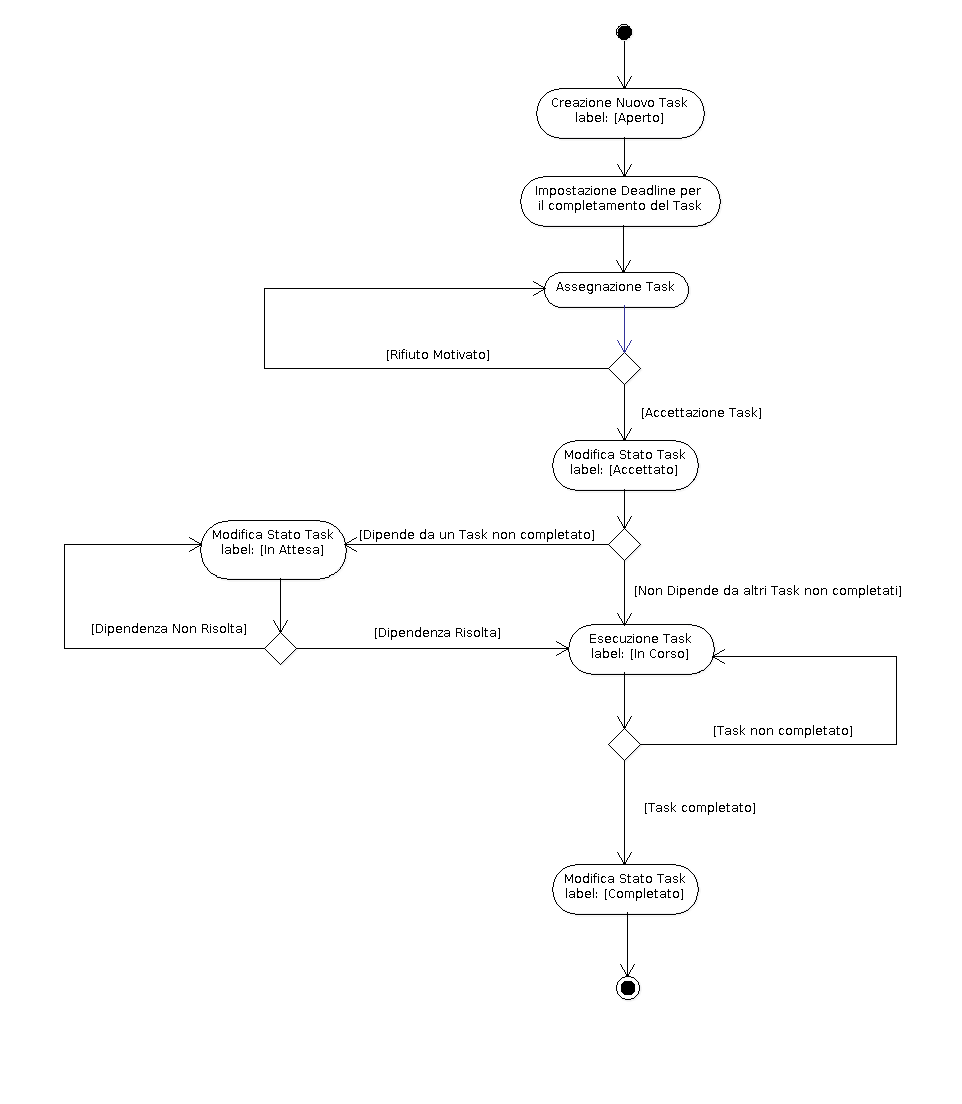
\includegraphics[scale=0.4]{ticketing.png}
\caption{Diagramma di gestione dei Ticket.}
\end{figure}
\end{center}

\subsubsubsection{Ticket di Verifica}

Per ogni \textit{\gloss{task}} marcato da etichetta \textbf{Completato} deve esserne verificata la correttezza e l'effettivo completamento attraverso la seguente procedura:
\begin{enumerate}
	\item Al completamento di un \textit{\gloss{ticket}} il \PM{} deve creare un \textit{\gloss{task}} marcato dall'etichetta \textbf{Verificare} ed assegnarlo ad un \VR{};
	\item Il \VR{}, nel caso riscontri anomalie o errori deve creare i \textit{\gloss{task}} necessari alla correzione degli stessi. Nel caso dell'assenza di errori il \VR{} chiude il \textit{\gloss{task}} e ne modifica lo stato impostando l'etichetta \textbf{Verificato}.
	\item Il \PM{} assegna gli eventuali \textit{\gloss{task}} creati dal \VR{} ponendo particolare attenzione a non far sorgere conflitti di interesse.
\end{enumerate}
 


\begin{center}
\begin{figure}[h]
\centering
\label{f2-Ticket Verifica}
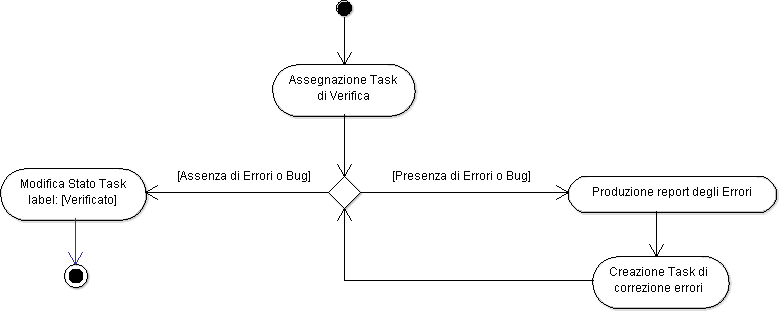
\includegraphics[scale=0.5]{ticketVerifica.png}
\caption{Diagramma di gestione dei Ticket di Verifica.}
\end{figure}
\end{center}

\subsubsection{Versioning} %Scelta di Git come sistema di Versioning
Come sistema di versionamento è stato scelto di usare \gloss{Git}. I motivi principali che ne hanno determinato la scelta sono:
\begin{itemize}
\item è gratuito e non proprietario
\item è un repository distribuito con la possibilità di commit e revert locali
\item è cross-platform
\item possiede un'abbondante ma semplice documentazione
\item è già stato usato da alcuni elmenti del gruppo
\end{itemize}

\subsubsection{Repository} %Scelta di Git come sistema di Repository, Spiegazione albero delle directory 
Viene creata una \gloss{repository} su github all'indirizzo \textit{https://github.com/lordnikolai/starware.swe15}. Ogni membro deve clonare la repository in locale da riga di comando tramite il comando \texttt{git clone}.
\paragraph{Commit}
Il comando per fare un commit è \texttt{git commit -a -m "<messaggio>"}. Il commit va fatto solo in uno stato consistente del documento modificato, dove per consistente si intende che non vi siano porzioni di testo interrotte o codice non completo. Il messaggio da associare al commit è obbligatorio e deve esprimere in modo sintetico ma chiaro quale sia l'elemento che in cui si è concentrto il commit e quale delle seguenti sia stata fatta:
\begin{itemize}
\item Aggiunta di un nuovo elemento
\item Correzzione o modifica
\item Moglioramento o ampliamento
\end{itemize}
\paragraph{Pull}
è preferibile fare un pull ogni volta che si comincia a lavorare da locale. Si raccomanda di controllare sempre il branch a cui si sta lavorando
\paragraph{Push}
Ogni volta che si ha un commit con informazioni che potrebbero interessare ad altri membri del gruppo bisogna fare una push della repository sulla directory online. Controllare che il commit rispetti le regole del paragrafo precedente.
\newpage

\end{document}
